\documentclass[a4paper,twoside,kulak]{kulakreport} %options: kul or kulak (default)

\usepackage[dutch]{babel}
\usepackage{pdfpages}

\faculty{Wetenschap \& Technologie Kulak }
\group{Ingenieurswetenschappen}
\title{Smart City}
\subtitle{Probleemoplossen en Ontwerpen Deel 2}
\author{Groep 6}
\institute {Aaron Vandenberghe, Dieter Demuynck, Jolien Barbier\\  
	Mathis Bossuyt, Rani Jans en Sarah De Meester \\~\\ 
	o.l.v. Benjamin Maveau Kevin Truyaert en Martijn Boussé} 
\date{Academiejaar 2020 -- 2021}
\address{
   KU Leuven Kulak           \\
   Wetenschap \& Technologie \\
   Etienne Sabbelaan 53, 8500 Kortrijk             \\
   Tel.\ +32 56 24 60 20     \\
  
   }

\begin{document} % hier begint de eigenlijke inhoud van het document
%Wat allemaal in het doc verwerkt moet zitten:
%-klantenvereisten
%-ontwerpsspecificaties
%-ontwerpskeuze
%-financieel rapprot
%-evaluatie wat gedaan is en wat nog moet gebeuren en hoe
%-wat nog verbeterd kan worden aan ontwerp

\titlepage 
\tableofcontents
\renewcommand\thesection{\arabic{section}}
\renewcommand\thesubsection{\thesection.\arabic{subsection}}
\newpage
\section*{Inleiding}\label{Inleiding}
%probleemstelling
%Ontwerpsproces en planning
Vandaag de dag zijn zelfrijdende auto's een actueel thema. Heel wat bedrijven zoals Tesla, BMW en Mercedes zijn volop bezig met de ontwikkeling van deze autonome wagens. Dit vanwege de vele voordelen. Een zelfsturende auto heeft namelijk een veel snellere reactie dan mensen. Hierdoor zullen ongevallen vermeden worden. Bovendien zullen er ook minder files zijn, waardoor er een mogelijke oplossing ontstaat voor de mobiliteitsproblemen. Daarnaast kiest een autonome auto voor de kortste weg. Hierdoor legt de auto minder kilometers af. Dit betekent dat deze soort auto's zowel instaan voor verkeersveiligheid als voor een meer milieubewust autotransport \cite{AutonomeAutos1, AutonomeAutos2}. De moeite waard dus om deze revolutionaire vooruitgang onder de loep te nemen en zelf ermee aan de slag te gaan.\\
Voor dit project betekent dit dat een zelfsturend autootje in staat moet zijn zich volgens een voorgeprogrammeerde route door een modelstad te bewegen. Dit is het idee van de `Smart City'. Deze `Slimme Stad' is een stad waarbij informatietechnologie gebruikt wordt om de stad te beheren en te besturen \cite{SmartCity}. Doorheen deze route, zal de auto verschillende obstakels tegenkomen. De bedoeling hierbij is dat deze hindernissen worden herkend en een bijpassende actie wordt uitgevoerd. Hoe dit kan worden geïmplementeerd zal aan bod komen in dit verslag. Daarnaast wordt het ontwerpproces uitvoerig uitgelegd. Hierin wordt het aanschaffen van onderdelen en de vereisten toegelicht.


\section{Klantenvereisten} \label{Klantenvereisten}
De klant wil dat de auto op een parcours lijnen kan volgen en stoppen aan een stoplijn. Een verkeerslicht moet ook kunnen geïnterpreteerd worden. Het autootje moet ook andere wagens kunnen detecteren en stoppen als deze te dicht komen, om aanrijdingen te vermijden.

\section{Hardwareontwerp} \label{Hardwareontwerp}

\subsection{Ontwerpspecificaties} \label{Ontwerpspecificaties}
%Een van de basisonderdelen is het chassis. Op dit onderdeel zal alles worden gemonteerd. Het is als het ware de ruggengraat van de auto.%wikipedia chassis
%Opdat de auto kan rijden zijn uiteraard wielen nodig. In het model dat verder wordt beschreven, worden er twee reguliere ronde wielen gebruikt en één kogelwiel. Om de aandrijving van de wielen mogelijk te maken wordt er aan ieder rond wiel een microtandwielmotor geplaatst. De regeling van de motoren gebeurt via de dual drive motor. Om uiteindelijk geheel de auto te laten voortbewegen is er een nood aan een hardwarecomponent namelijk een microcontroller. Deze fungeert als een soort mini computer. Daarnaast zal ook extra stroomtoevoer moeten worden voorzien. Hiervoor worden twee oplaadbare lithium-ion batterijen gebruikt. Verder is het ook nuttig om gebruik te maken van een breadboard. Dit is echter geen onderdeel van de zelfrijdende auto, maar is handig voor het testen van elektrische circuits.


De modelstad bestaat uit enkele straten en 25 identieke kruispunten. De straten zijn telkens 1 meter lang. Op het parcours met grijze ondergrond zijn er twee soorten zwarte lijnen te vinden: volglijnen en stoplijnen. Op het kruispunt zelf zijn er geen lijnen. Het autootje zal deze lijnen moeten kunnen interpreteren en een onderscheid kunnen maken tussen deze twee soorten. Het verschil tussen deze twee lijnen zit hem in de dikte. Volglijnen zijn 25 mm dik, stoplijnen 50 mm. De auto moet de lijnen van 25 mm dik volgen en stoppen bij de lijnen van 50 mm dik \ref{fig:plattegrond}. Het moet dus een sensor bevatten die deze lijnen kan herkennen, meer bepaald een reflectiesensor. De auto komt een stoplijn tegen bij het naderen van een kruispunt. Hier zal het moeten stoppen en een verkeerslicht moeten interpreteren. Het feit dat het verkeerslicht om 7.5 cm hoogte staat, speelt een rol bij het bepalen van de hoogte van de auto. De auto moet dus voorzien zijn van een kleurensensor of een camera die de twee verschillende kleuren van het stoplicht kan onderscheiden. Bij een rood licht moet de auto blijven stil staan aan de stoplijn, bij groen moet hij weer starten.

%Smalle auto
\begin{figure}
	\centering
	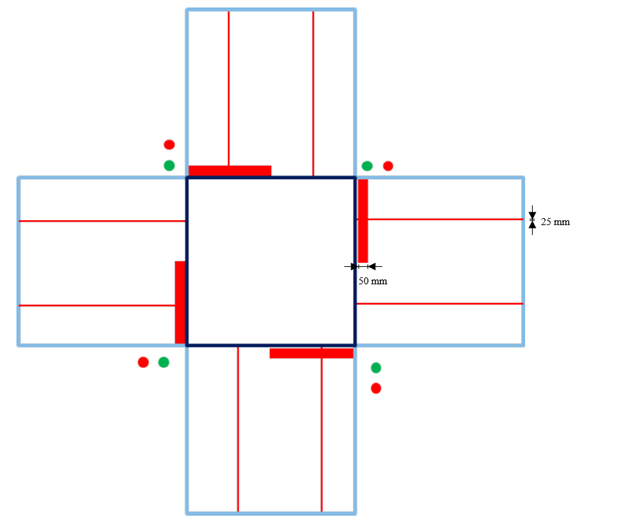
\includegraphics[width=.6\textwidth]{volglijnenEnStoplijnen}
	\caption{Kruispunt}
	\label{fig:plattegrond}
\end{figure}

Ook moet het wagentje voorgaande wagens kunnen detecteren en stoppen wanneer deze te dichtbij komen. Als de wagen van achter wordt aangereden is dit niet zijn fout, dus enkel voorliggers kunnen een probleem vormen. Om andere wagens te herkennen moet het wagentje een afstandssensor bevatten die voorliggers detecteert en vervolgens een signaal verzendt zodat de motoren vertragen om een botsing te voorkomen. Er moet dus ook gezorgd worden voor een zo kort mogelijke remafstand.

Verder moet de auto aan een aanvaardbare snelheid voortbewegen. De tandwielmotoren rond de wielen zorgen voor de aandrijving. Daarbij is het belangrijk dat het een beperkte massa heeft, maximaal 500 gram. Dit zal ervoor zorgen dat het op een veilige manier zich aan ongeveer 10 cm/s kan voortbewegen zodat ook de remafstand beperkt blijft.

Ten slotte moet men vanop afstand kunnen ingrijpen wanneer er iets fout loopt, zoals een aanrijding. Zo zal de auto bestuurbaar gemaakt worden vanuit een toetsenbord.



%Per onnderdeel verwijzen voor bibliografie!!!

%- herkennen lijnen: welke soort sensor (bv reflectie voor lijnen)
%- stoplicht: kleurensensor, tot stilstand komen blabla
%- snelheid: massa belangrijk
%- andere wagens detecteren => remafstand, massa belangrijk => stoppen door signaal zodat motoren vertragen
%- op afstand ingrijpen


\subsection{Ontwerpskeuze}
%Zeer specifiek toelichten waarom je elk onderdeel heb gekozen.
\label{Ontwerpskeuze}

\subsubsection{Chassis}
Als eerste wordt de chassis besproken. Voor deze auto wordt een rechthoekige variant gebruikt met als afmetingen 80 mm op 172 mm  \cite{RobotChassisRechthoekigZwart}. 
% 3 figuren invoegen assemblage (Mathis)
Deze is handig in gebruik wegens de verscheidene groottes van de groeven. %groottes of vormen?
Bovendien is de rechthoekige vorm zeer gemakkelijk om alle componenten van de auto vast te hechten. Een ronde chassis zoals bijvoorbeeld is hiervoor minder geschikt \cite{RobotChassis}. Ook zijn er in deze laatste groeven aanwezig voor de wielen. 
Dit impliceert dat er minder ruimte is om andere onderdelen te assembleren op het onderstel. %nadeel nog vermelden over onze 
%motordrivers die er niet aan gesoldeerd konden worden?
\label{Chassis}

\subsubsection{Wielen}
Een goede keuze voor de wielen zijn die met respectievelijk een diameter en dikte van 42 mm en 19 mm.
Figuur \ref{fig:wiel} geeft een idee hoe ze eruit zien.

\begin{figure}
	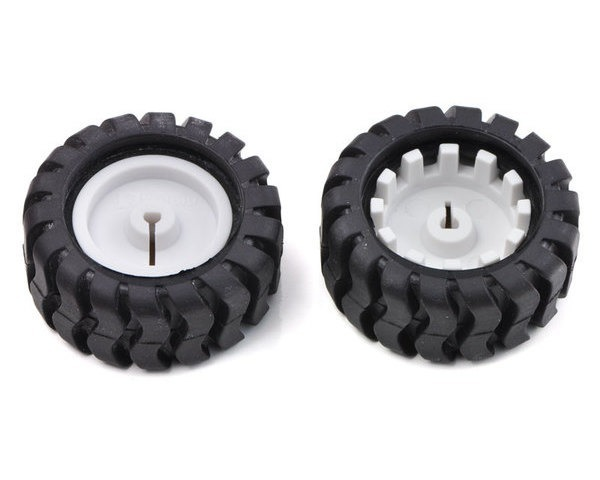
\includegraphics[width=0.5\textwidth]{wielen}
	\centering
	\caption{Wiel met diameter 42 mm en dikte 19 mm} 
	\cite{Wiel42x19mm}.
	\label{fig:wiel}
\end{figure}

De dikte van dit wiel is geschikt om voldoende grip te hebben. Bij dunnere banden is er dus minder grip en dat zou ervoor kunnen zorgen dat de auto niet snel genoeg kan remmen bij obstakels en stoplijnen \cite{Banden}. Daarnaast is de diameter evenredig met de versnelling en de nodige kracht.
Een kleiner wiel impliceert namelijk een kleinere kracht en een kleine versnelling. Een groot wiel daarentegen levert een grote versnelling maar heeft een grote kracht nodig. Het is dus belangrijk dat de middenweg wordt genomen om een goede snelheid te behalen zonder al te veel moeite.  

De auto van dit project is een driewieler. Dit heeft enkele voordelen. Eerst en vooral is dit eenvoudiger om te draaien. Als je vier wielen hebt, zijn er twee vaste punten en dus meer wrijving waardoor de auto minder vlot kan draaien. Om af te slaan is het makkelijker om één vast punt te hebben en dat de andere wielen eromheen draaien.
Ten tweede reduceert een driewieler de kosten van het project. Een vierde wiel was niet nodig dus zou het niet verstandig zijn om aan het te kopen. Zo is er ook nog marge in het budget voor eventuele wijzigingen tijdens het project. Idealiter wordt als derde wiel gebruik gemaakt van een kogelwiel. We kozen voor het kogelwiel omdat dit flexibelere draaibewegingen heeft dan een normaal wiel. 
\label{Wielen}


\subsubsection{Motoren}
Aansluitend hierbij spelen de tandwielmotoren ook een belangrijke rol. Motoren met een groot tandwiel starten zeer gemakkelijk maar behalen geen al te grote snelheid. Kleine tandwielen hebben dan weer de omgekeerde eigenschap. Het is dus van belang dat er een tandwielen worden gebruikt met een gemiddelde grootte namelijk de motor met verhouding 50:1. Niet alleen de grootte speelt een rol, maar ook de kracht van de motor. Hiervoor wordt het best gekozen voor de "High Power" (HP). Deze motoren hebben een grote efficiëntie.%dan welke?
Een bijkomend voordeel is het gewicht dat slechts 9,5 gram bedraagt \cite{MicroMetalGearMotor50:1HP}. %Erbij zetten dat het ook een groter vermogen heeft?
Hoe minder de onderdelen wegen, hoe minder kracht je nodig hebt om de auto te laten rijden. 

Door het gebruik van deze motoren is er nood aan motorbeugels zodat de ze aan de chassis  vastgemaakt kunnen worden. Aangezien de motoren een breedte van 12 mm en een hoogte van 10 mm hebben, is het logisch dat de beugels met afmetingen 12 mm op 10 mm worden genomen \cite{MicroMetalGearMotorBeugel}.
Verder is een dubbele aandrijfmotor essentieel om de tandwielmotoren met de microcontroller te verbinden. In dit project wordt gekozen voor de Dual Drive DRV8833 \cite{DualDriveDRV8833}. 
\label{Motoren}


\subsubsection{Microcontroller}
De microcontroller is cruciaal voor de werking van de auto. Het zorgt ervoor dat het autootje de taken correct uitvoert. De keuze van de microcontroller gaat in dit project naar NI MyRIO in plaats van Raspberry Pi \cite{nimyrio},\cite{RaspberryPi}.
Dit is omdat deze zowel met analoge als digitale signalen kan werken. 
%Dit heeft enkele gevolgen. 
%Eerst en vooral hebben de inputs de mogelijkheid om een digitaal of een analoog signaal door te geven. 
Bij Raspberry Pi zijn er enkel digitale inputs beschikbaar. Dit heeft implicaties voor de keuze van de sensoren, waarvoor ik verwijs naar het onderdeel over sensoren in \ref{Sensoren}.
Daaruit volgt dat alles in LabVIEW geprogrammeerd wordt.
%Ten tweede zal alles in LabVIEW worden geprogrammeerd.
Deze software en microcontroller zijn ervoor gemaakt om samen te werken. Dit biedt veel voordelen tijdens de implementatie. In sectie \ref{Implementatie} wordt hier dieper op ingegaan. %verwijzing nog aanpassen want Sarah ging dat stukje veranderen.
Daarnaast heeft dit ook invloed op de keuze van het chassis. Achteraf viel het op dat de microcontroller niet paste op het chassis waardoor men het heeft vastgemaakt met makerbeams.
%Waarom voor deze microcontroller gekozen: prijs en deze kan met analoge signalen

\label{Microcontroller}

\subsubsection{Sensoren}
Zoals al aangehaald is, wordt in dit ontwerp gewerkt met een reflectiesensor en een afstandssensor. Er bestaan twee soorten, namelijk sensoren met digitale output en met analoge output. Zoals hierboven verteld is, kunnen beiden gebruikt worden met de NI MyRIO. De analoge sensoren geven meer info dan de digitale. De digitale kunnen maar één of twee signalen doorgeven aan de microcontroller namelijk nul of een. Ofwel staat de sensor aan ofwel uit. De analoge sensoren geven analoge signalen. Dit soort signaal kan alle waarden aannemen, in tegenstelling tot een digitaal signaal. Langs de andere kant zorgen de analoge sensoren voor meer programmeerwerk \cite{DigitaalOfAnaloog}. Voor dit project is het beter dat de informatieoverdracht tussen sensor en microcontroller vlot verloopt met behulp van echte waarden. Bij keuze van een analoge sensor is dit dus voldaan, alhoewel er meer programmeerwerk bij komt kijken. %echte waarden nog wat uitleggen wat ermee bedoeld wordt. experimentele waarden?
De reflectiesensor zal onderaan de auto, dichtbij de grond geplaatst worden zodat de lijnen op het juiste moment zullen herkend worden. Ook is de reflectiesensor iets breder dan de volglijn. Zo zal het vanaf de auto bij een stoplijn komt, andere waarden binnenkrijgen.

~

Ook om de kleuren groen en rood te herkennen, is er nood aan een sensor of camera. Er is keuze tussen een Raspberry Pi-camera, webcam en kleurensensor voor het interpreteren van de stoplichten. In dit ontwerp wordt gekozen voor de kleurensensor. Deze is compatibel met de NI MyRIO en weegt maar 3,23 gram \cite{Webcam,TCS34725KleurSensorBOB}. Bovendien weegt de webcam 223,6 gram. Hoe minder de wagen weegt, hoe stabieler het is en hoe minder kracht het nodig heeft om een bepaalde snelheid te kunnen halen. De Raspberry Pi-camera is enkel bruikbaar met een Raspberry Pi als microcontroller. Aangezien in dit model wordt gewerkt met een NI MyRIO, is dit dus geen optie \cite{RPi-camera}. Samengevat: de kleurensensor heeft als voordeel dat het zeer licht is en compatibel is met de NI MyRIO-microcontroller. % 2 keer is? 
\label{Sensoren}


\subsubsection{LED-lampjes}\label{LED-lampjes}
Als extra optie om LED's te plaatsen omdat het ons het meest haalbaar leek in vergelijking met de andere ideeën. Eerst dachten we eraan om servomotoren te gebruiken maar deze waren schaars en ingewikkeld te modelleren waardoor er risico zou zijn dat het wagentje niet juist werkt.
%Gear-motor: niet 100, want anders veel toeren, maar te weinig kracht (50 omgekeerd)


\subsection{Assemblage}
%titel nog aan te passen
%Alles op elkaar zetten, 3D-modellen?
%NOG DOEN
Voordat het autootje fysiek geassembleerd wordt, werd dit eerst via de computer gedaan. Aan de hand van de reeds gemaakte 3D-modellen, werd een 3D-model van het autootje gemaakt. Doordat de apparte onderdelen van het autootje al af waren, moesten die enkel nog samengevoegd worden. Het 3D-model zie je in figuur
{\bf{\Large Moet nog ingevoegd worden/verwijzing naar figuur stap voor stap opbouw}}
Door dit model was het gemakkelijker om de wagen in elkaar te zetten omdat er naar iets toegewerkt werd en de plaatsing van de onderdelen zichtbaar was. Er wordt gestart met het chassis. Daar worden dan de motoren met wielen aan de onderkant opgeplaatst. Ook het kogelwiel wordt bevestigd aan de onderkant. Helemaal van voor wordt een steunpaal gezet. Aan de voorkant wordt de reflectiesensor onder de steunpaal vast gemaakt. Ook aan de voorkant maar dan vooraan op de steunpaal de afstandssensor bevestigd. Aan de zijkant van de paal wordt op een hoogte van 7.5 cm wordt de kleursensor bevestigd. Dit is aan de rechterkant vast gemaakt. Net achter de steunpaal wordt de {\it dual drive motor} geplaatst. Dwars op het midden van het chassis wordt de microcontroller bevestigd.



\label{Assemblage}

\section{Softwareontwerp}\label{Softwareontwerp}

Om te kunnen implementeren is het belangrijk om informatie in te winnen door opzoekingswerk. Het is dan ook cruciaal dat er specifieker wordt gezocht hoe het materiaal best gebruikt kan worden.
%bron myrio nog vermelden
Dit is nuttig om de communicatie tussen de sensoren en de NI MyRIO-controller te begrijpen. Ook de spanning dat nodig is om de sensoren te laten te werken is belangrijk. Zo zijn er enkele poorten die precies 5 volt leveren. Dit is perfect, aangezien dit compatibel is met het spanningsverschil van de sensoren. Vervolgens kan het elektrisch circuit opgesteld worden. Dit is handig om te weten welke onderdelen er met elkaar worden verbonden. Eenmaal dit in orde is, kan het programmeerwerk beginnen.
%Laatste twee zinnen nog aan te passen.

Voor het schrijven van stukjes code, is het ten sterkste aangeraden om over de onderdelen van de auto te beschikken opdat de fragmenten van de code kunnen worden uitgetest. In de subsectie die volgt wordt een korte analyse gegeven van de observaties die volgen uit kleine experimenten. Om de testen mogelijk te maken, moet er eerst contact worden gemaakt tussen een computer en de microcontroller. Dit kan gerealiseerd worden met de ´LED´ functie in LabVIEW. Eenmaal er connectie is, branden de lampjes op de microcontroller en kunnen de experimenten van start gaan.


\subsection{Experimenten}
\subsubsection{Signalen ontvangen en versturen}
Het doel van de eerste test is de communicatie met de microcontroller te begrijpen. Met behulp van het standaardprogramma \texttt{main.vi} in LabVIEW kan er gezien worden hoe de microcontroller beweegt.  
De tweede test bestaat uit het versturen en ontvangen van signalen. Om te weten wanneer een signaal verstuurd wordt, wordt volgend experiment uitgevoerd. Een draad wordt bevestigd tussen de poorten van 11 en 13 Ampère. Op het moment dat de draad kantelt en hierdoor op de \textbf{z-as meer dan 0,5 wordt weergegeven,}%nog extra uitleg vragen. 
wordt er een signaal ontvangen door de poort van 13 A. Van hieruit wordt een nieuw signaal verstuurd maar dit keer naar de computer. Bijkomend is dit experiment nuttig om te begrijpen hoe er kan gedebugd worden. Bovendien is het cruciaal voor de verdere implementatie van de auto.  


%%% moet taalonafhankelijk in het verslag dus enkel stukken van de code mogen erin. 
%Het echt programma zal bestaan uit verschillende subVI's. Zo zullen we een stukje code schrijven dat specifiek is voor het detecteren van wagens die voor ons rijden. Als er een obstakel minder dan 20 cm voor ons staat zal hij moeten stoppen of de snelheid aanpassen. Een ander stukje code zal het lezen van het stoplicht zijn. Hier zal de microcontroller de signalen van kleursensor moeten interpreteren. Een ander deel zal met de reflectie sensor de volglijn volgen en weten wanneer die overgaat in een stopstreep waarna het wagentje moet stoppen. 
%Er zal ook een deel zijn over het kruispunt. Dit zal bestaan uit drie delen. Deze zijn rechtdoor rijden en links of rechts afslaan. Hieraan zullen de richtingsaanwijzers gekoppeld worden.  

\subsubsection{Sensoren}
Met behulp van voorbeeldprogramma's is het mogelijk om de gekregen data die van de sensoren te interpreteren. Zo is er een idee met welke waarden er moet gewerkt worden in het definitief programma. 

Een eerste experiment is met de reflectiesensor. Deze sensor werkt met een programma dat de acht waarden teruggeeft. 
Een van de vereisten voor het autootje is een lichte en donkere kleur te onderscheiden. Om te weten welke waarden de sensor geeft, kan dit worden getest met een wit papier, de zwarte voorkant van een laptop en een grijs tafelblad. Bij het papier wordt een waarde dichtbij 1 verkregen terwijl bij het donkere spectrum waarden tussen 4 en 4,5. %en de tafel?
Door het experimentje is er nu geweten welke waarden er moeten gebruikt worden om de lijn op de grond te kunnen volgen.
% !!!!!!!! Eventueel hetgene hieronder weglaten?? Is dit noodzakelijk voor het verslag????
% We hebben het aantal waarden dat we krijgen per seconde wat vermindert van 1000 naar 100 om op die manier stabielere inputs te krijgen. Anders was het moeilijk om die waarden te lezen.

Het volgende experiment is met de afstandssensor. Bij deze test wordt een voorwerp eerst ver van de sensor gehouden en dan dichterbij. Bij afstanden kleiner dan 80 cm worden lage waarden bekomen zoals 0,1. Afstanden groter dan 80 cm geven een negatieve waarde. Wanneer de afstand echter op een tiental cm van de sensor verwijderd is, wordt een maximale waarde van 3 verkregen. Eenmaal de lengte tussen de afstandssensor en het voorwerp kleiner is dan 10 cm, zakt de geleidelijk aan naar 2. De conclusie van deze test: voor de afstandssensor zullen de waarden twee en drie moeten gebruikt worden.

\subsection{Definitieve programma's}
%manuele override
%inlezen sensoren
%programma auto niet botsen -> stopwaarde



\section{Discussie} %discussiesectie 
\subsection{Resultaten demo} 
Nog te schrijven. 

\subsection{Financiële kant} 
In het financieel rapport \ref{financieel rapport} krijgt men een beeld van wat er is aangekocht en hoeveel eenheden hieraan zijn besteed.  

In dit project kreeg elke groep 3500 eenheden om te bieden en onderdelen te bestellen voor de auto. Bij de eerste bestelling werden in totaal 1615 eenheden uitgegeven. Na de bieding, waaraan 1350 eenheden werden gespendeerd, bleven er nog 535 eenheden over. Deze 535 eenheden werden besteden aan de mechanische stukken en draden. 



\section{Besluit}
Nog te schrijven.

%Samenvatting wat in verslag
%Conclusie: werkte goed of niet
%Future outlook: wat zou je nog doen als je nog weken extra had, verbetering


\newpage

\section{Bijlagen}
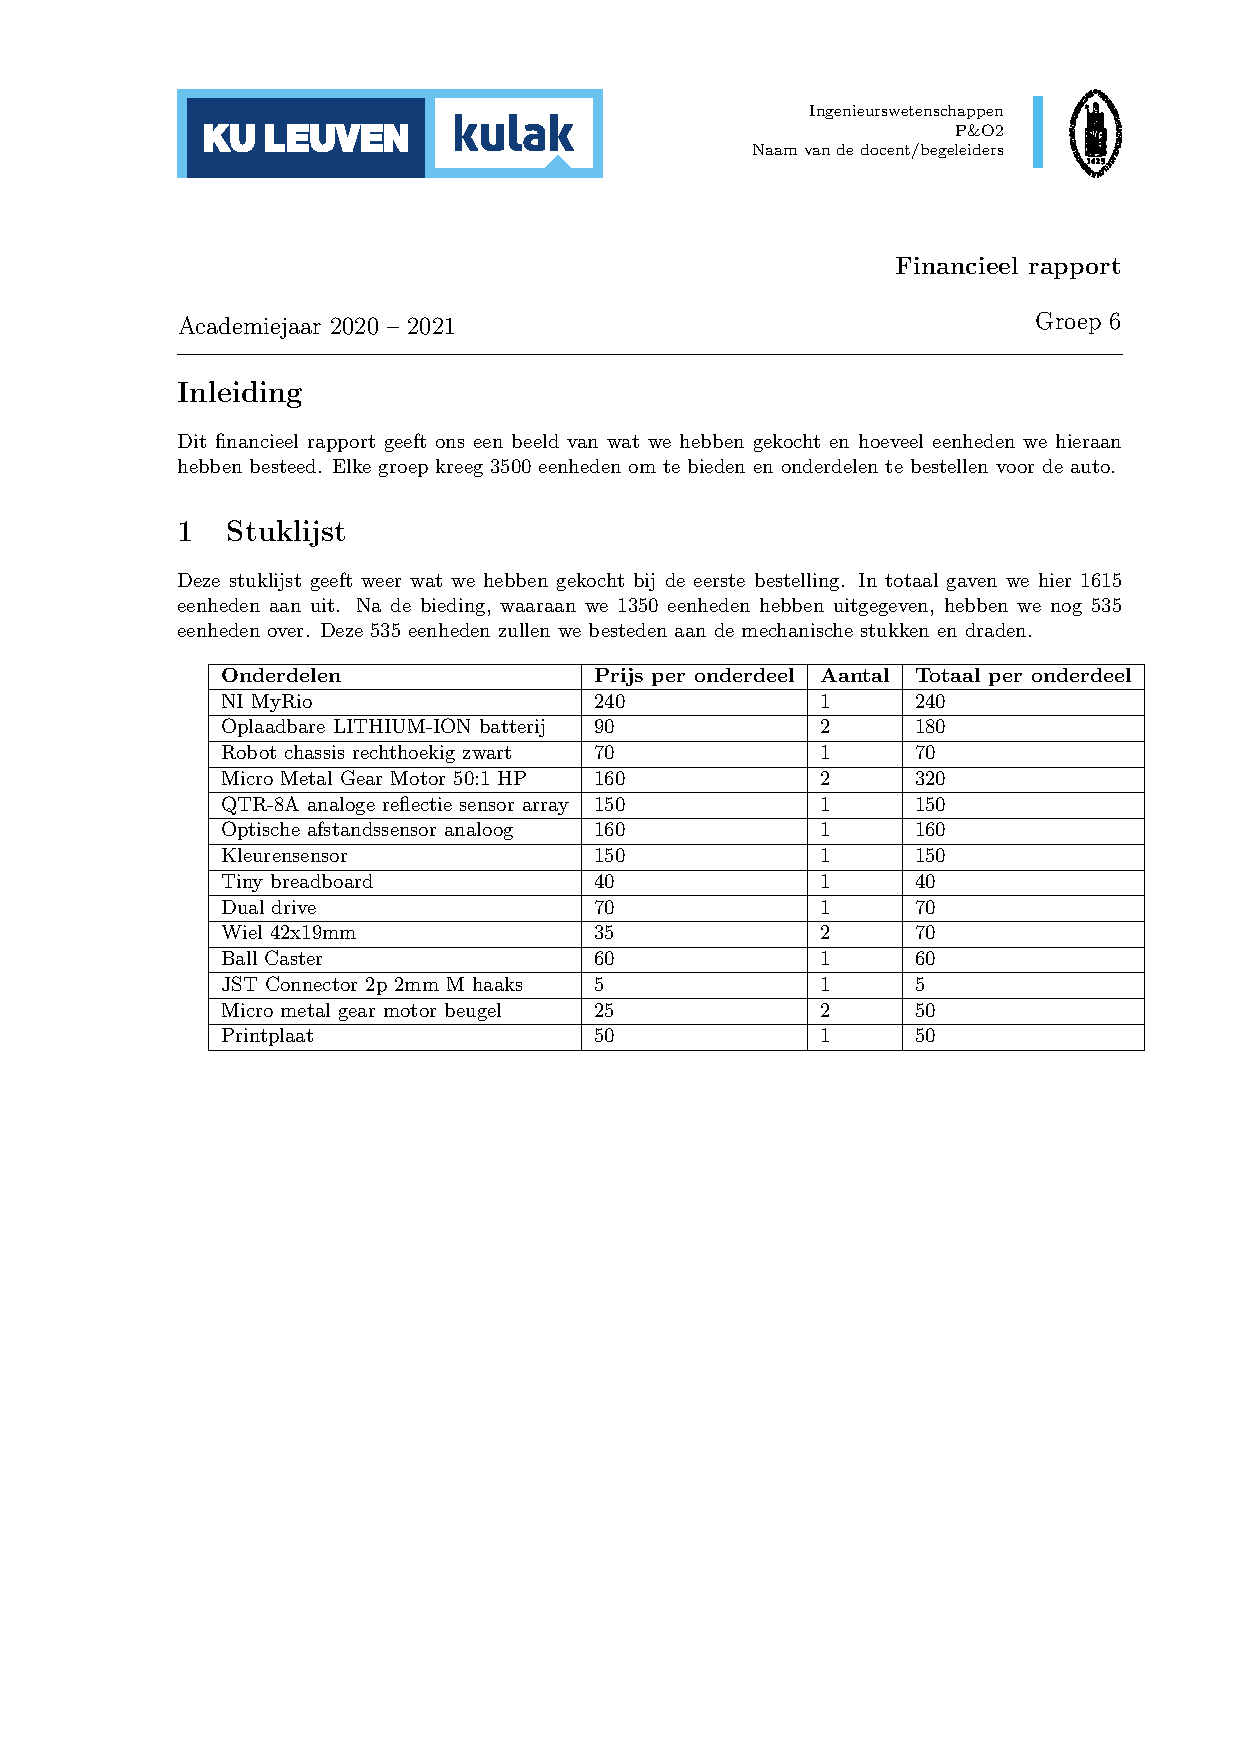
\includepdf{FinancieelRapport.pdf}\label{financieel rapport}
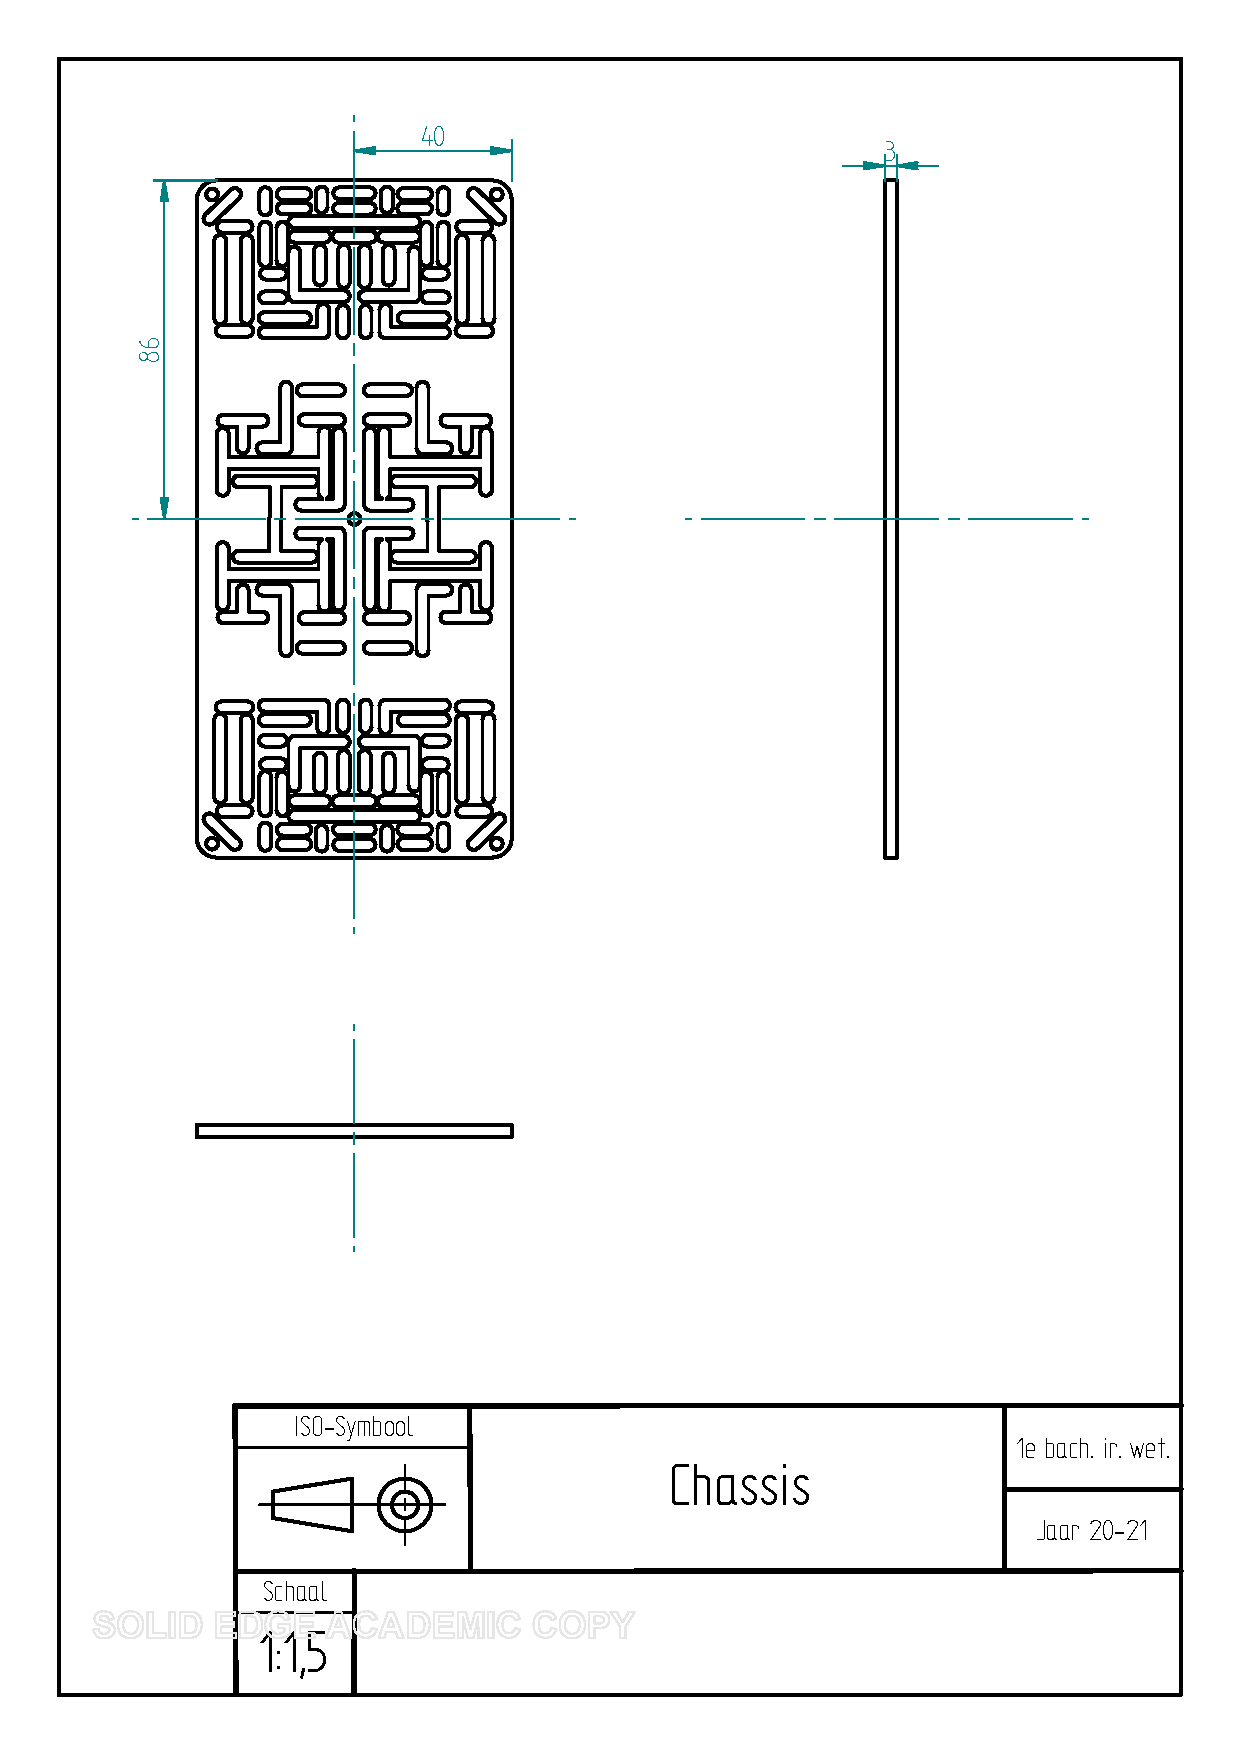
\includepdf{TechnischeTekeningChassis.pdf}\label{TechTekChassis}
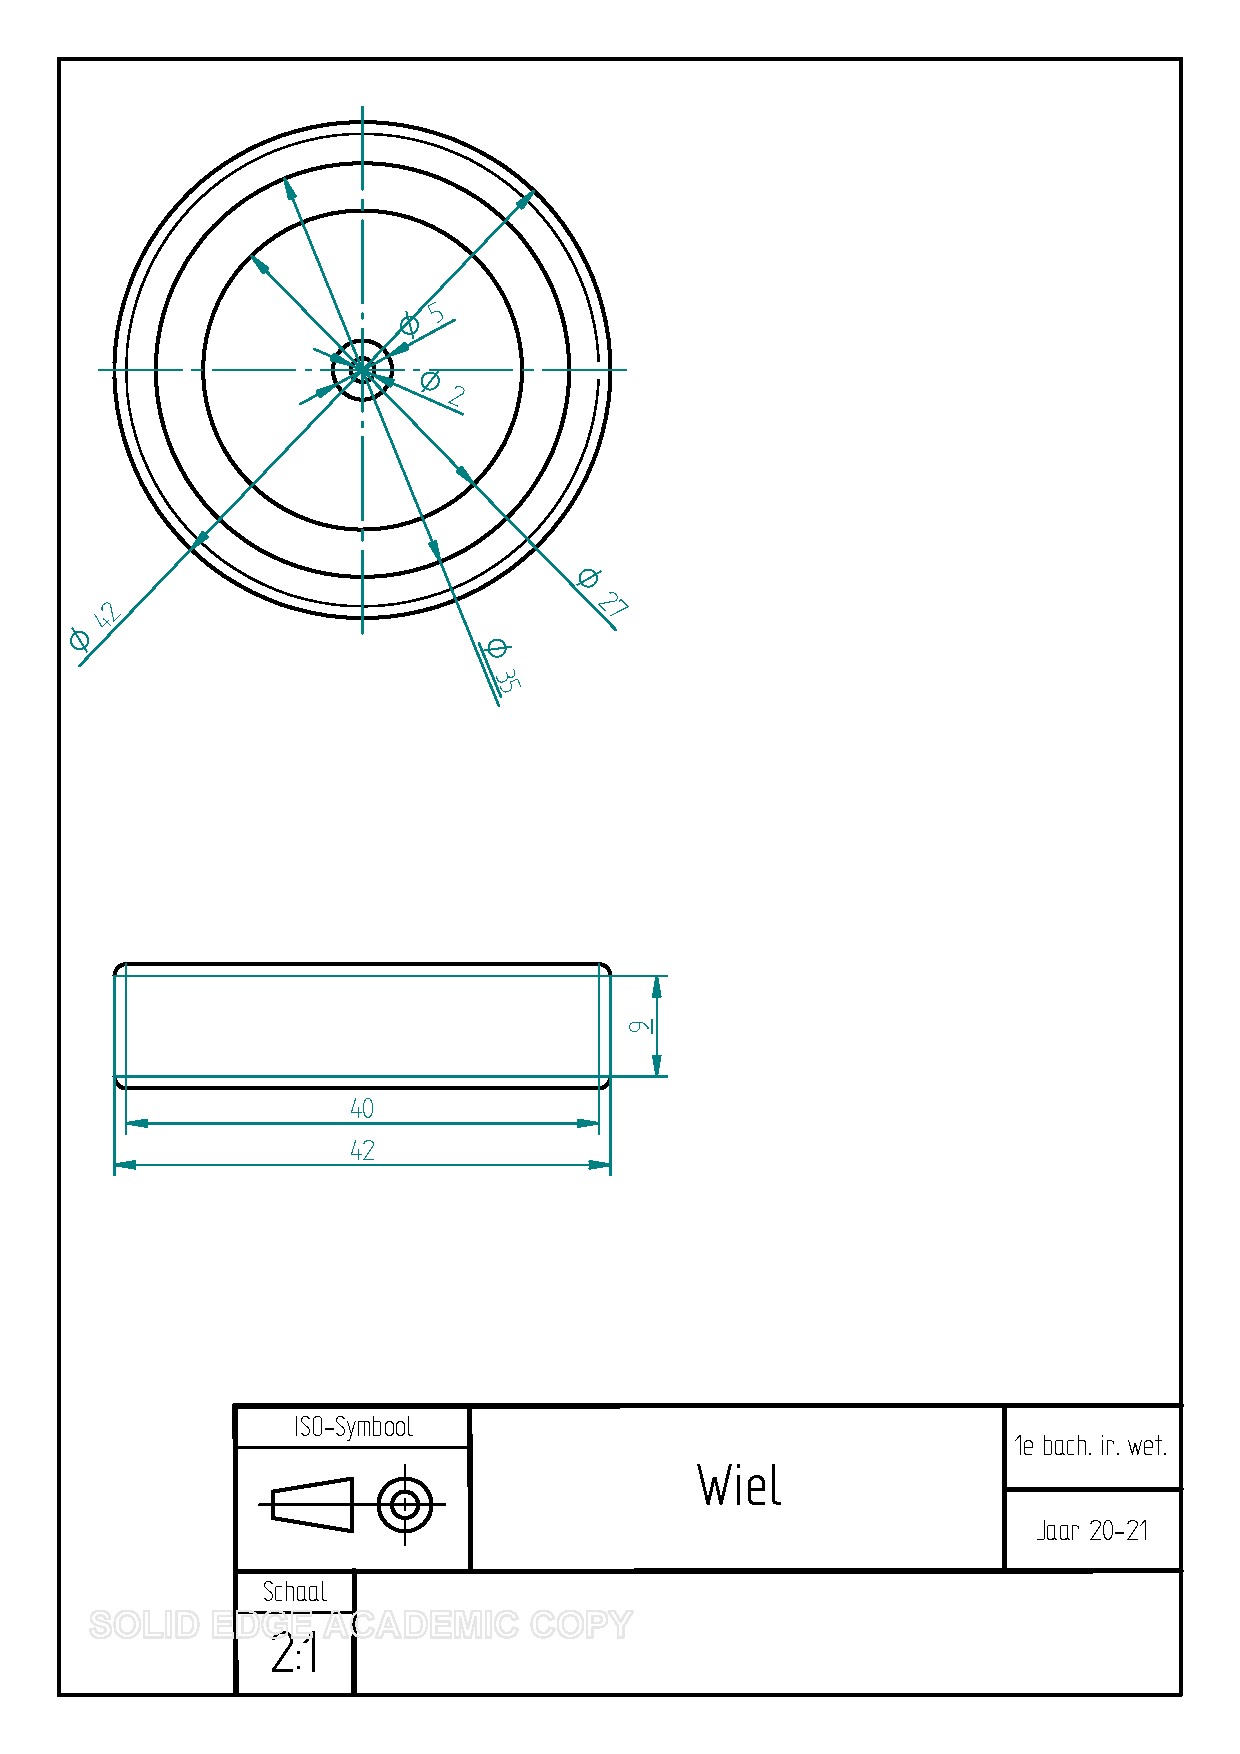
\includepdf{TechnischeTekeningWiel.pdf}\label{TechTekWiel}
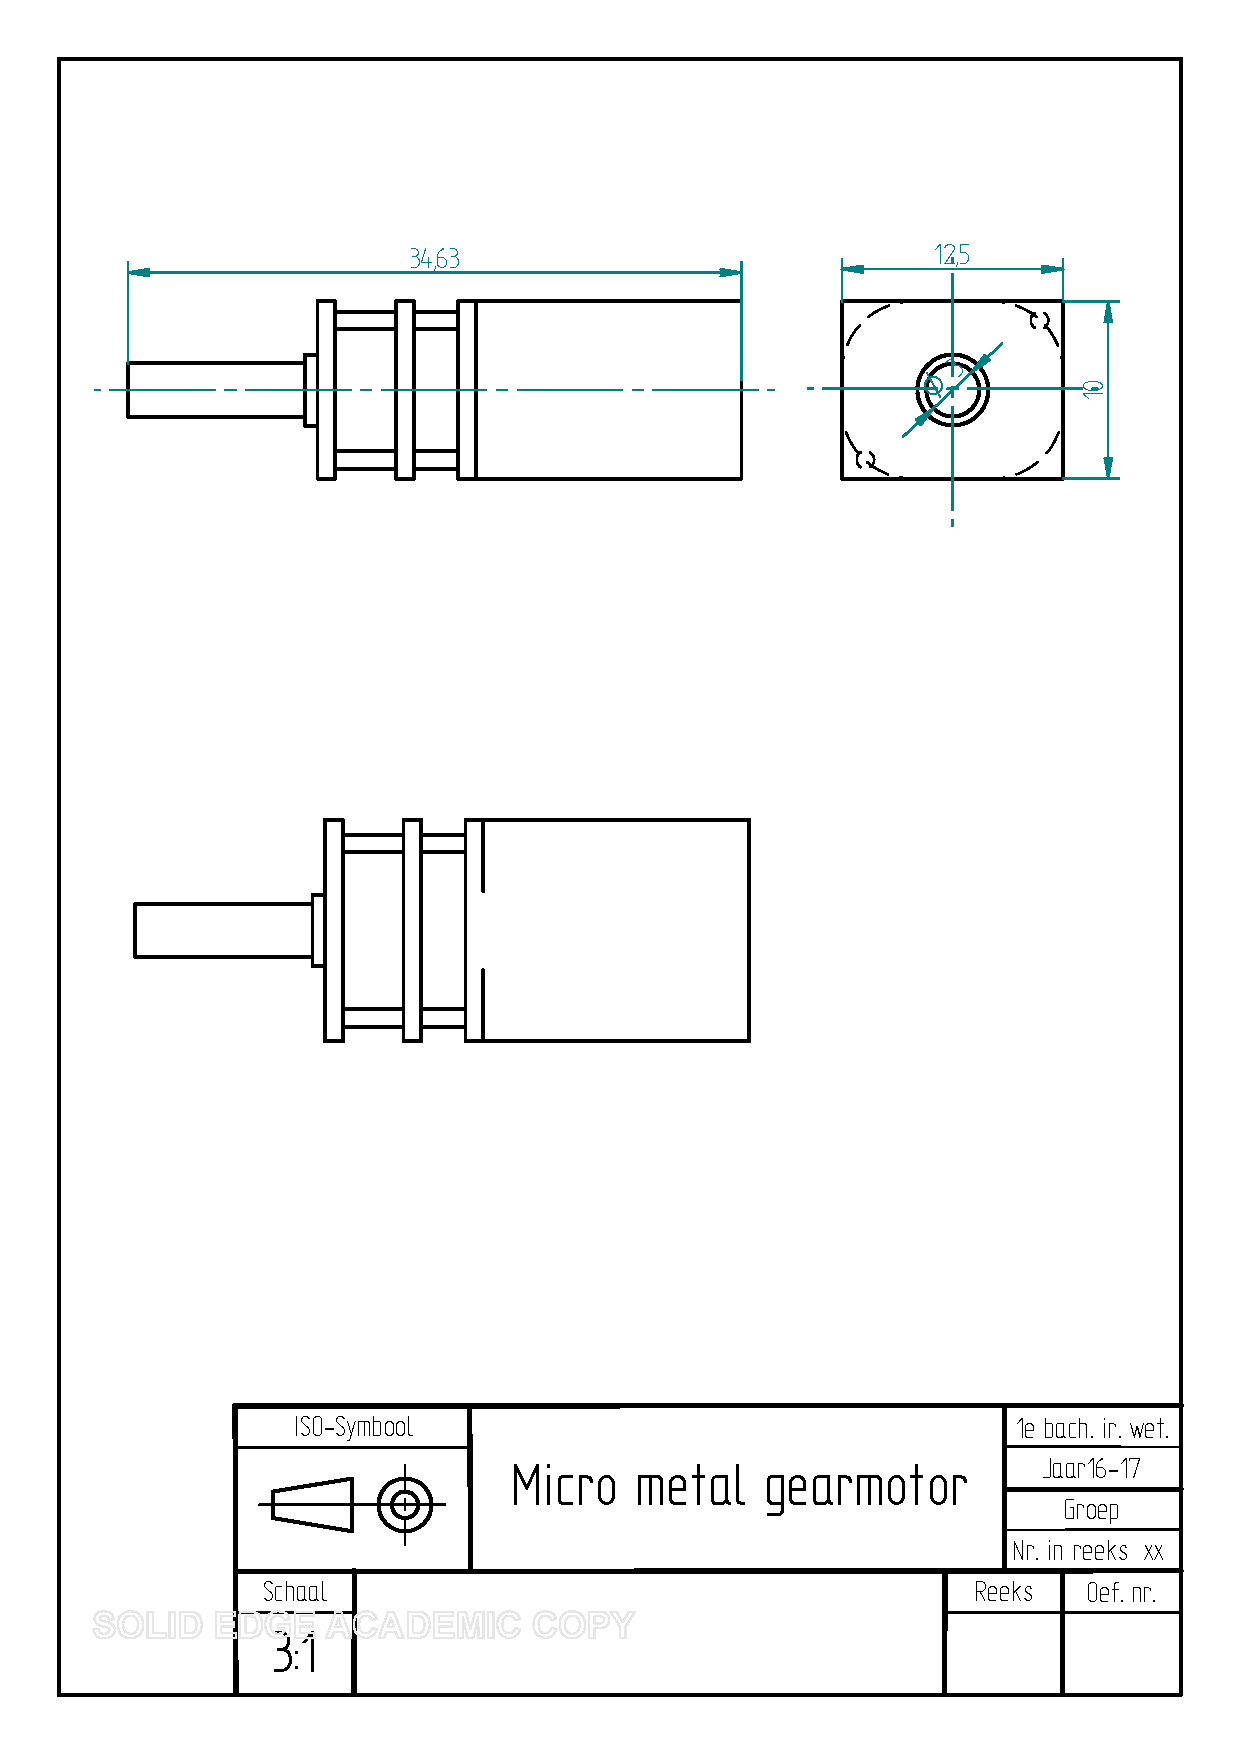
\includepdf{TechnischeTekeningMotor.pdf}\label{TechTekMotor}
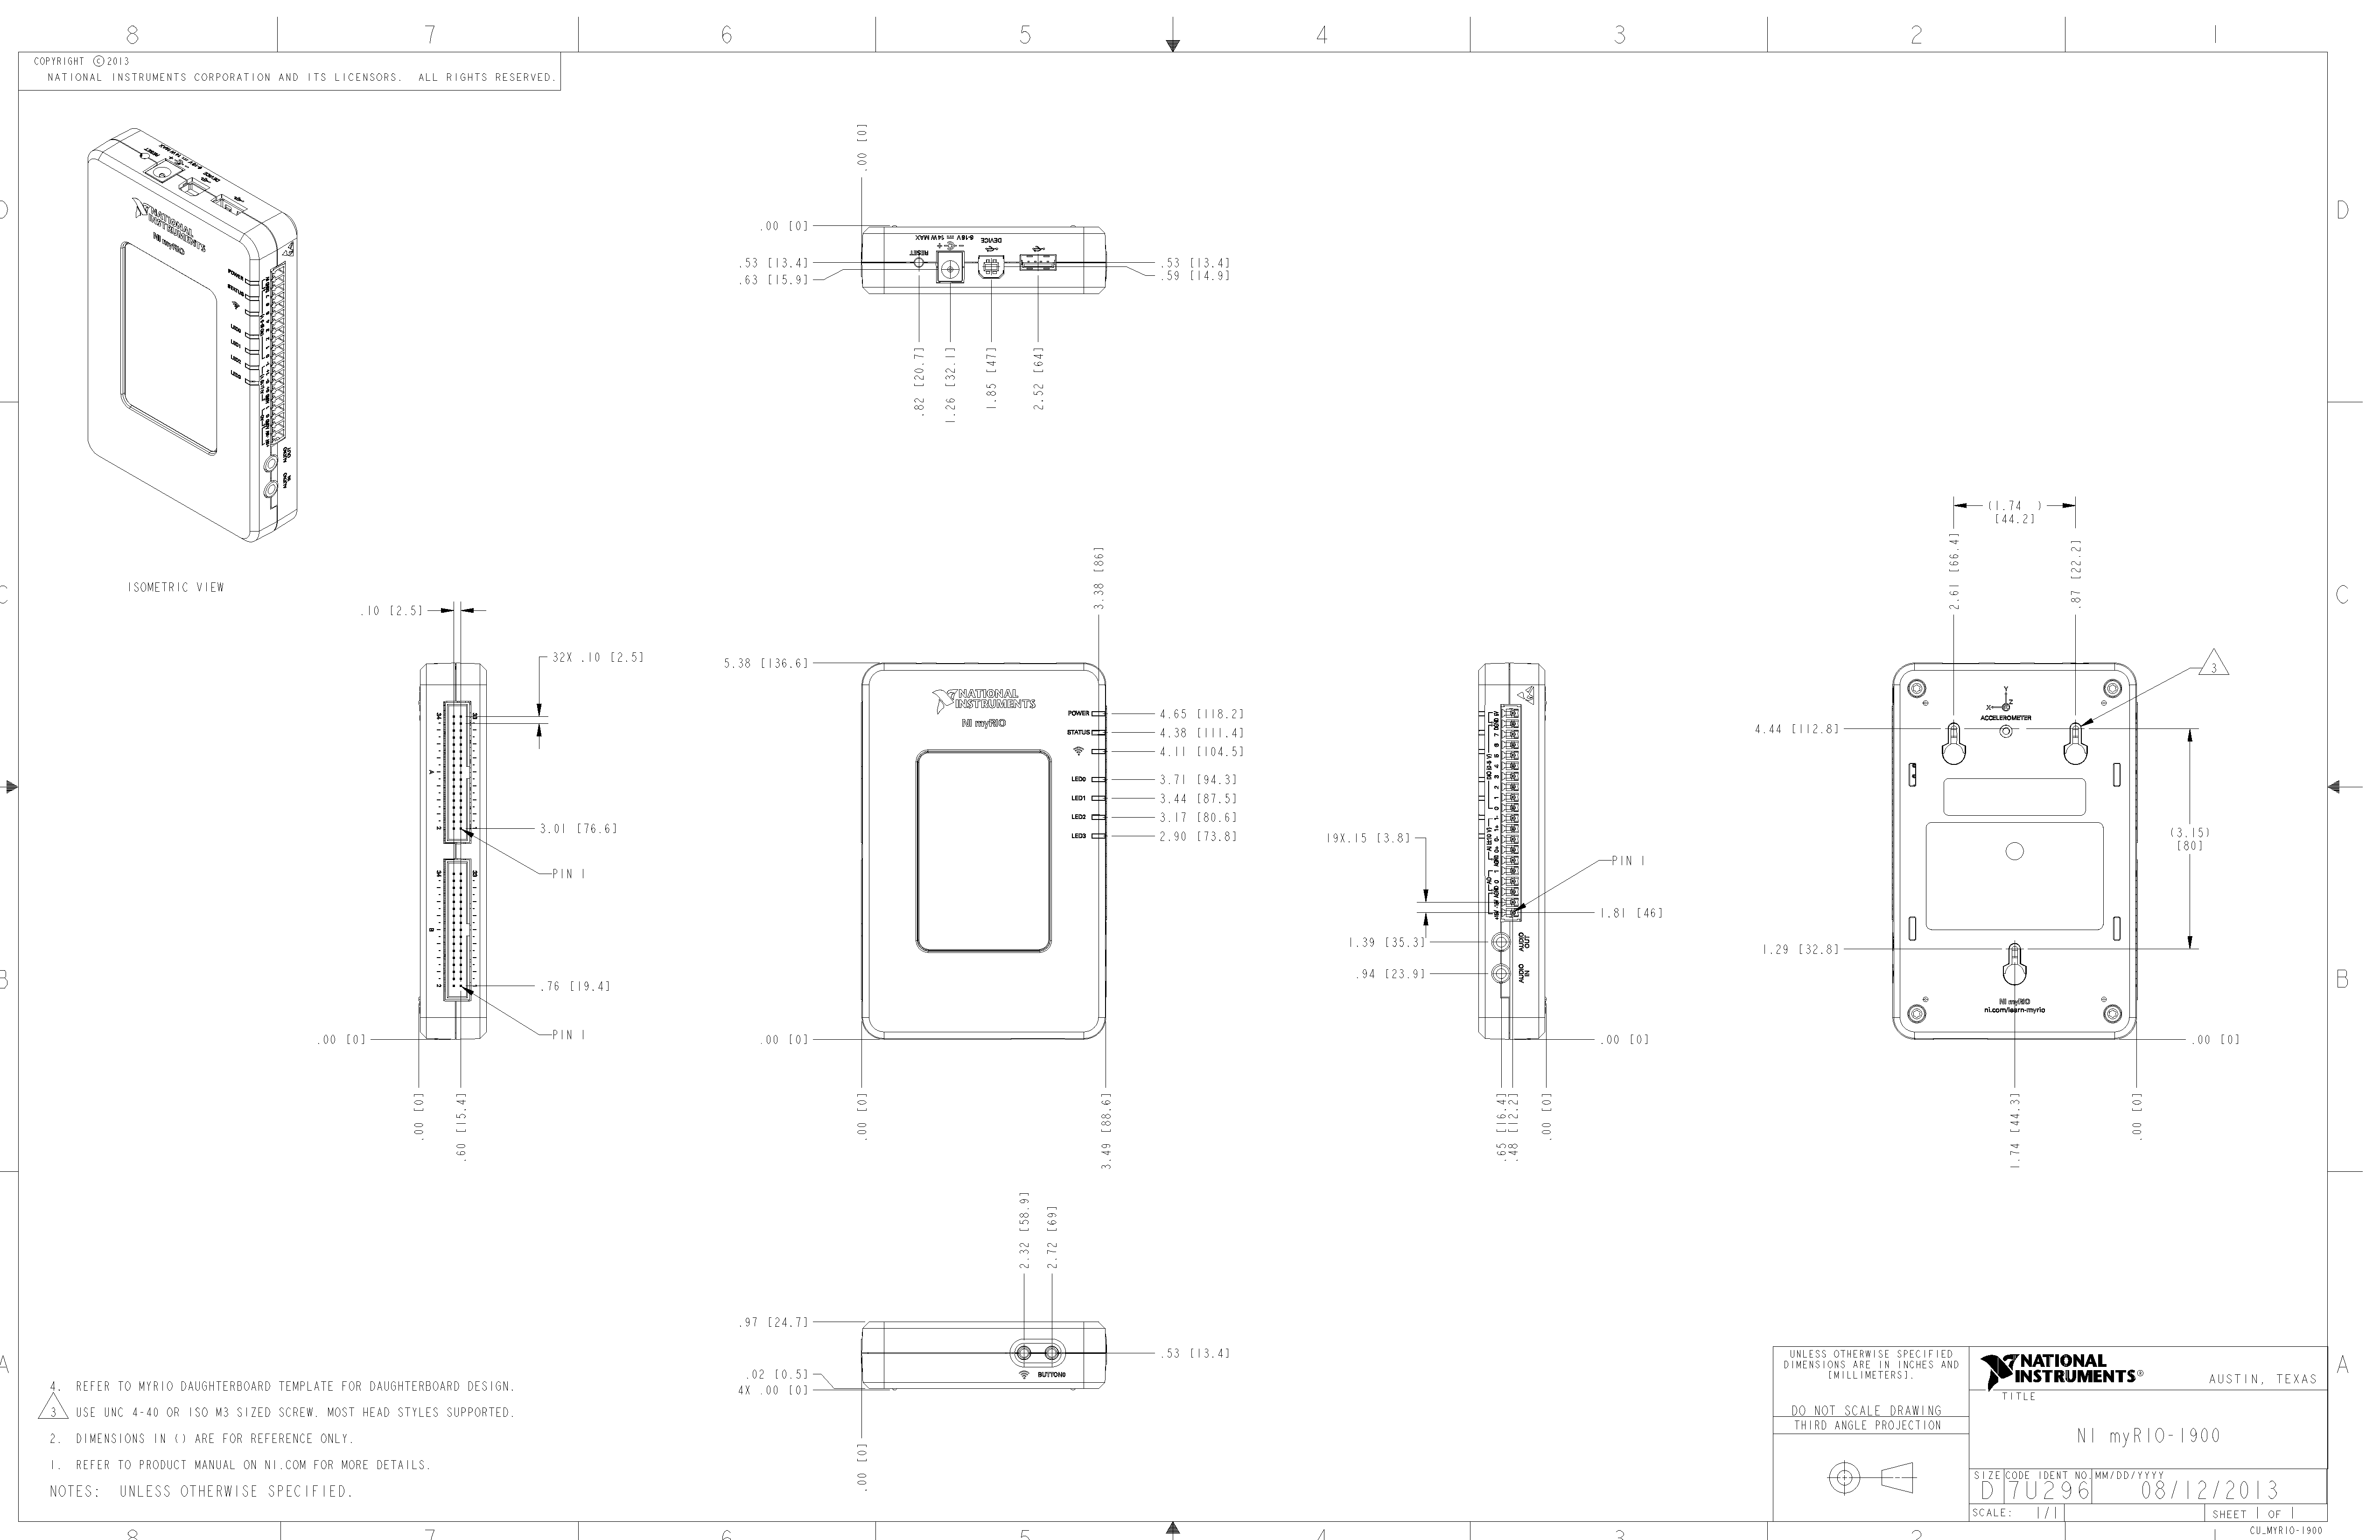
\includepdf{TechnischeTekeningMicrocontroller.pdf}\label{TechTekMicrocontroller}
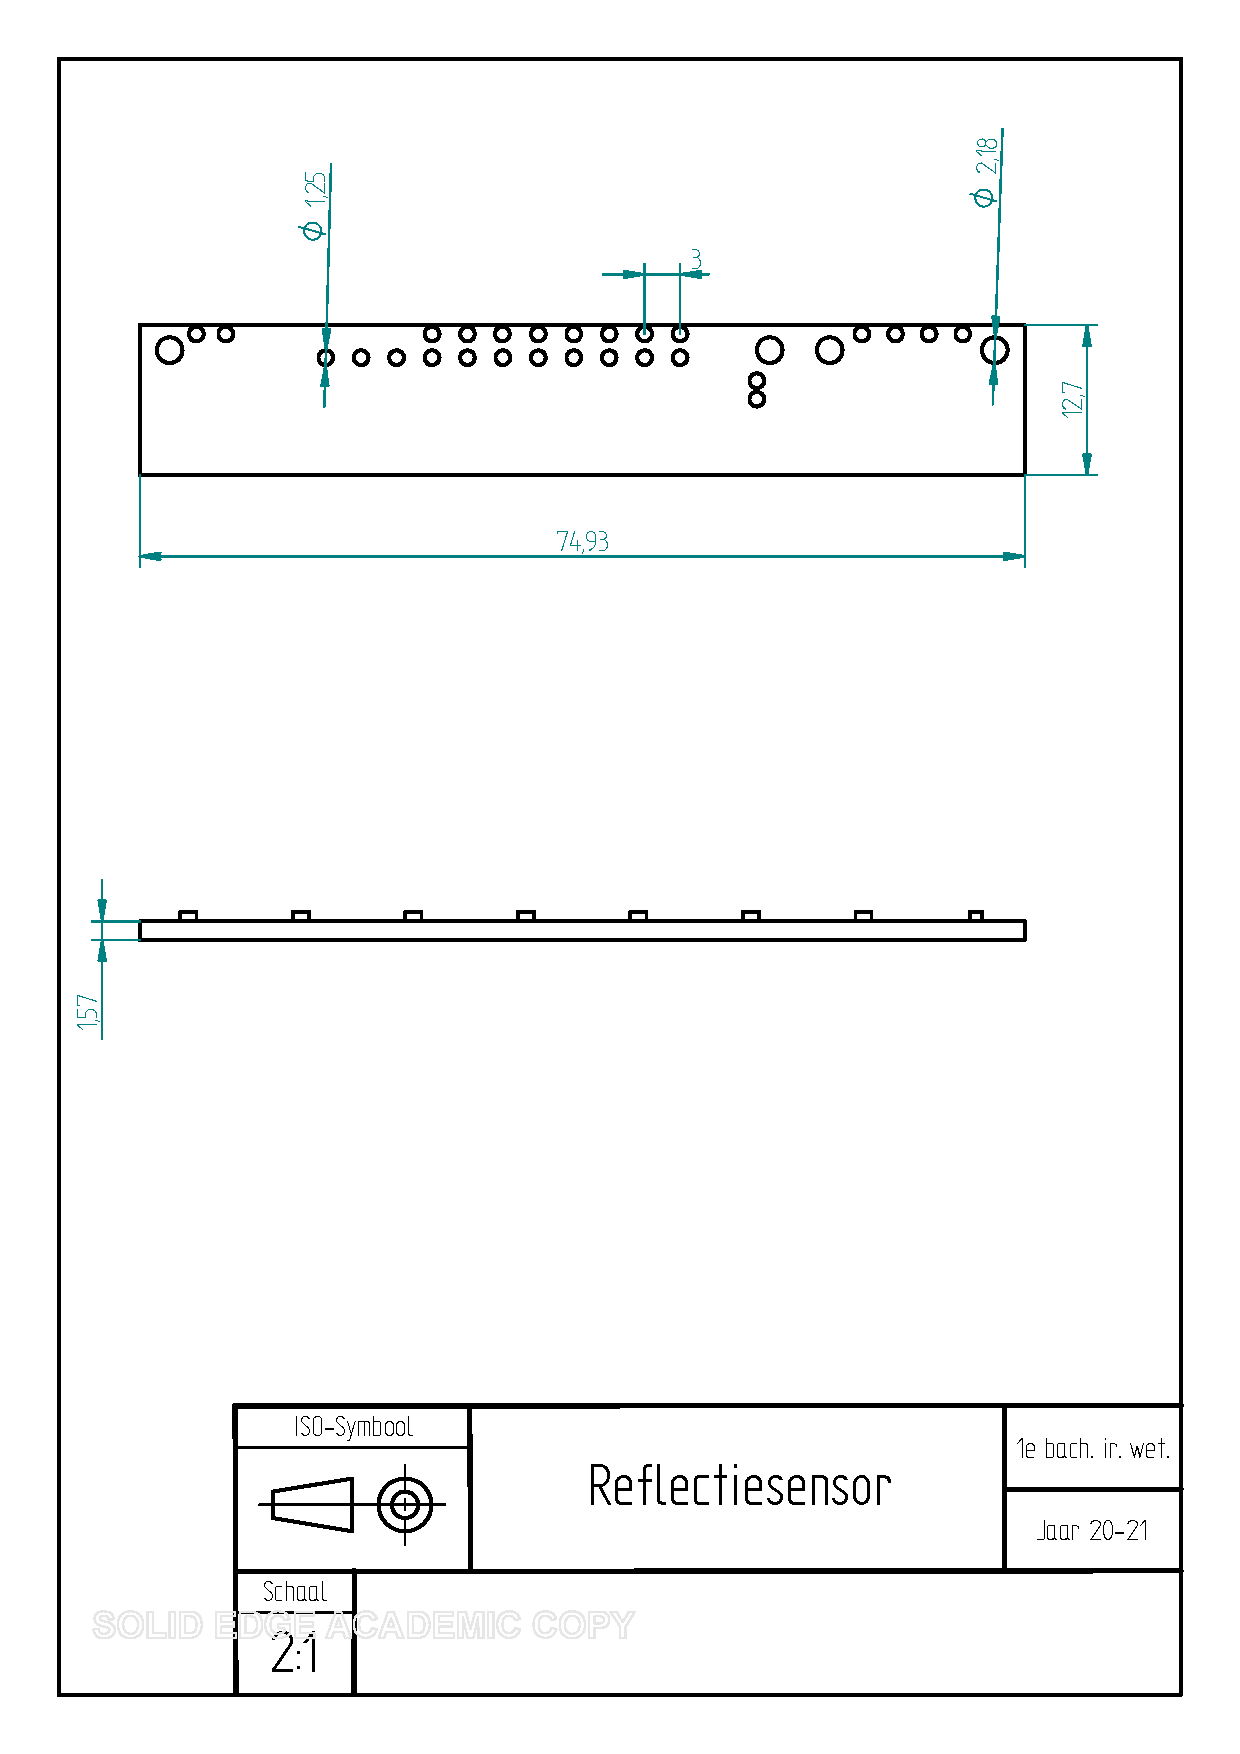
\includepdf{TechnischeTekeningReflectiesensor.pdf}\label{TechTekReflectiesensor}
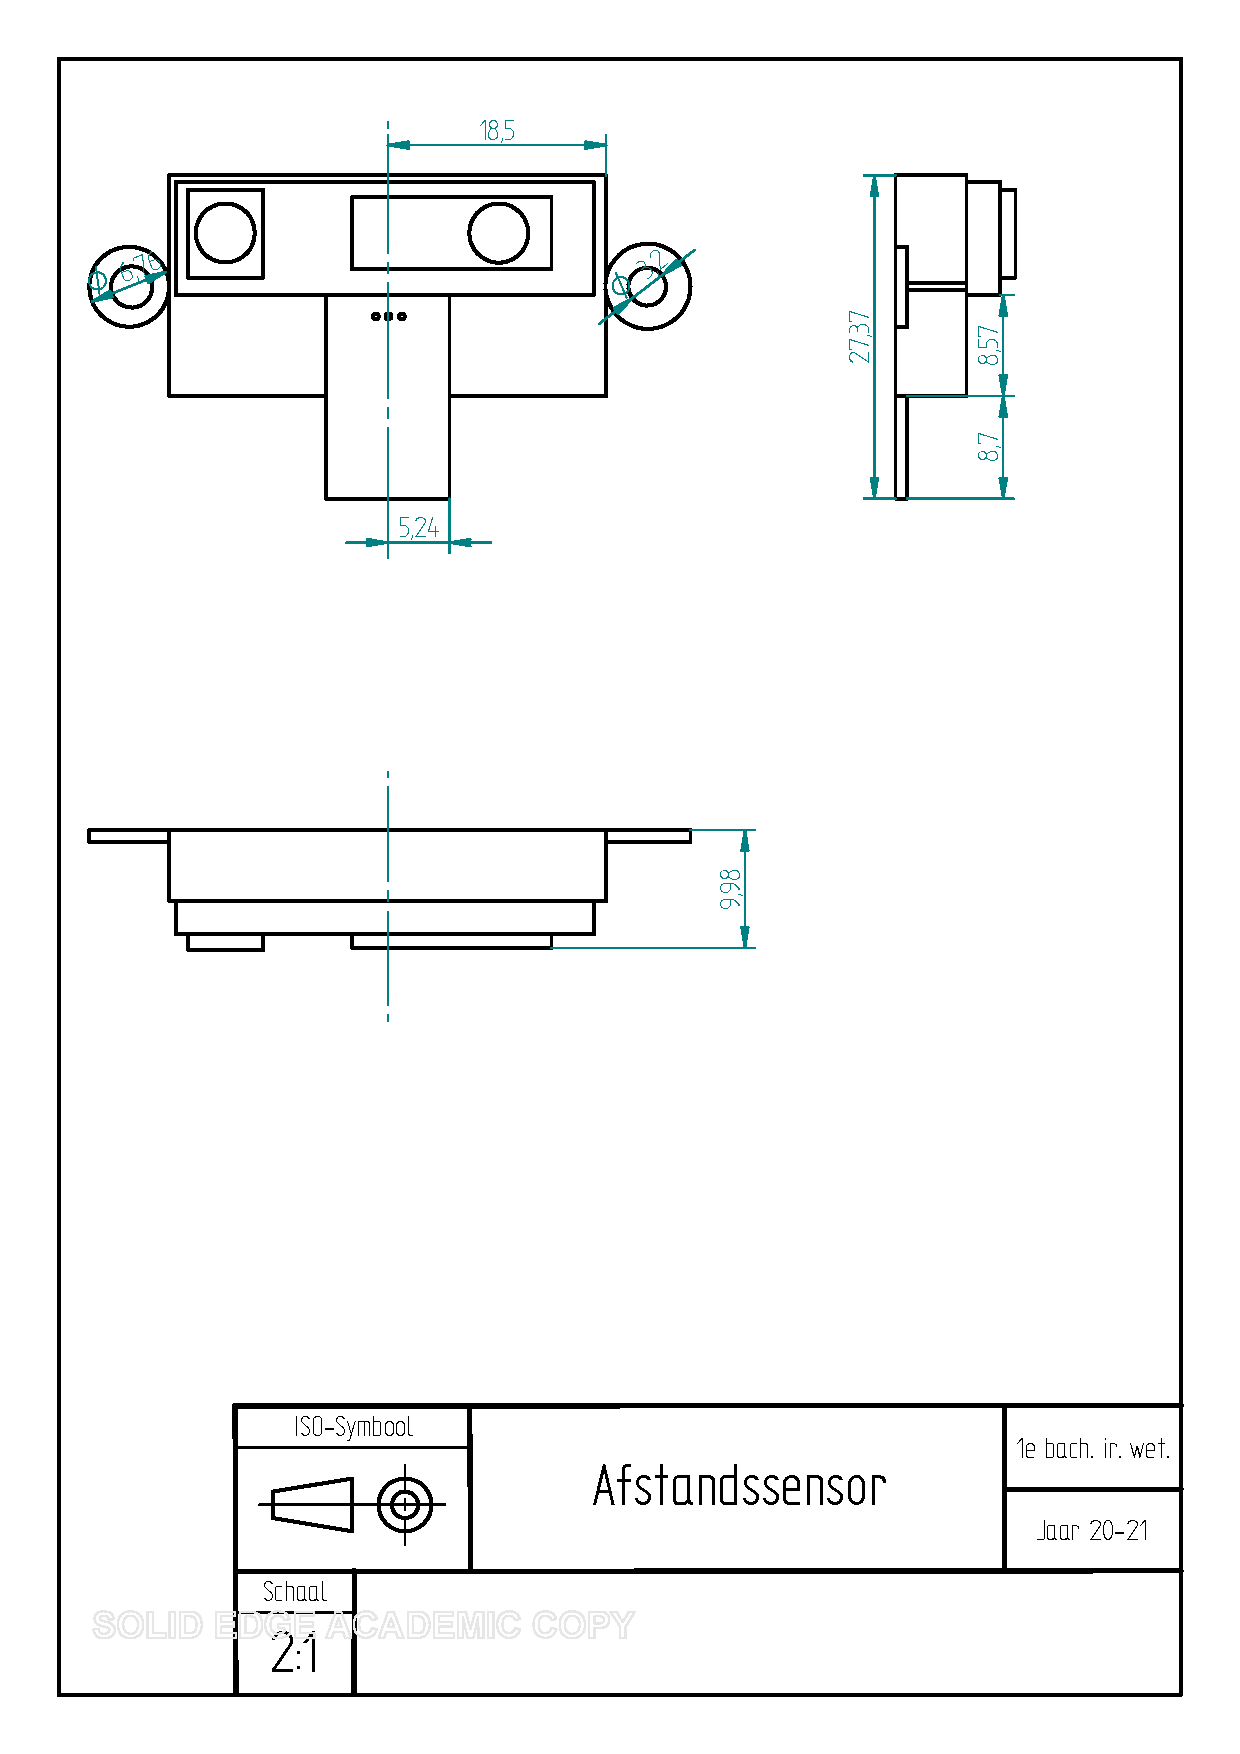
\includepdf{TechnischeTekeningAfstandssensor.pdf}\label{TechTekAfstandssensor}
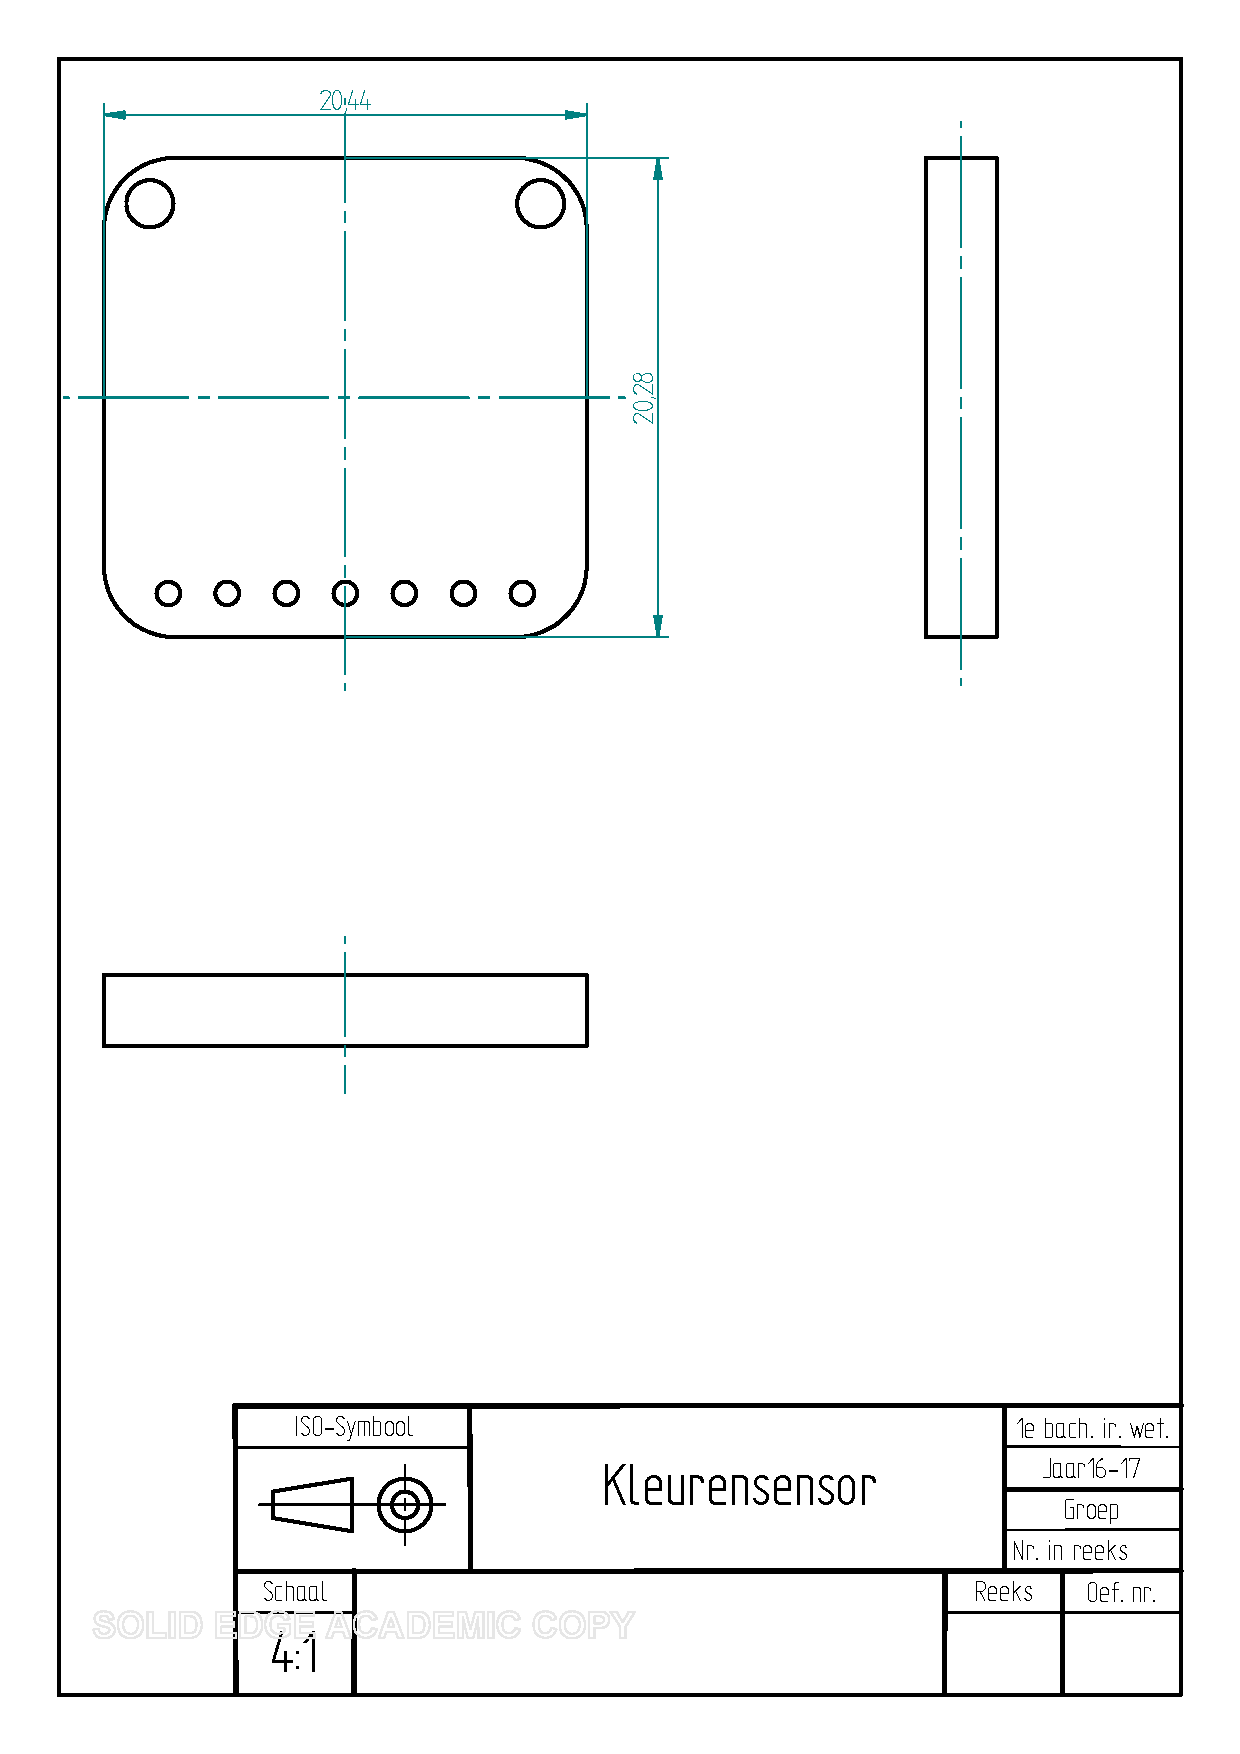
\includepdf{TechnischeTekeningKleurensensor.pdf}\label{TechTekKleurensensor}




\bibliographystyle{plain}
\bibliography{bronnen_verslag}
\bibliographystyle{unsrt}
\end{document}
